\documentclass[10pt, twocolumn]{article}

\usepackage[utf8]{inputenc}
\usepackage[T2A]{fontenc}
\usepackage[russian]{babel}

\usepackage{indentfirst}
\usepackage{amssymb, amsfonts, amsmath, mathtext}
\usepackage{graphicx}
\usepackage{float}

\makeatletter
\setlength{\@fptop}{0pt}
\makeatother

\title{Поиск собственных чисел и функций краевой задачи}
\author{Коновалов Андрей, 073}
\date{}

\begin{document}

\maketitle

\section{Постановка задачи}

Рассмотрим краевую задачу на собственные значения для обыкновенного дифференциального уравнения второго порядка
\begin{equation} \label{eq:bvp}
\begin{aligned}
  y'' + (\lambda - x^2) y &= 0 \\
  y(0) = y(1) &= 0.
\end{aligned}
\end{equation}

Требуется найти все значения $\lambda \in [0, 20]$ такие, что задача допускает нетривиальное решение, а также численно построить эти решения.

\section{Общий метод решения}

Поскольку это уравнение второго порядка с неизвестным параметром $\lambda$, то для его решения требуется третье условие.
В силу линейности и однородности задачи \eqref{eq:bvp}, ее решение определяется с точностью до произвольного постоянного множителя, а значит третье условие можно задать произвольным образом.
Зададим его так:
\begin{equation*}
  y'(0) = 1.
\end{equation*}

Решать задачу будем методом стрельбы.
Соответствующая задача Коши записывается так:
\begin{equation} \label{eq:cp}
\begin{aligned}
  y'' + (\lambda - x^2) y &= 0 \\
  y(0) = 0, \; y'(0) &= 1.
\end{aligned}
\end{equation}

Решение $y(\lambda, x)$ задачи Коши будет зависеть от $\lambda$ и иметь невязку с правым граничным условием краевой задачи:
\begin{equation*}
  F(\lambda) = y(\lambda, 1) - y(1) = \delta.
\end{equation*}

Решение $y(\lambda, x)$ будет решением краевой задачи, если невязка $\delta = 0$.

Решив численно уравнение
\begin{equation} \label{eq:dis}
  F(\lambda) = 0,
\end{equation}
относительно $\lambda$ мы найдем собственные значения $\lambda$ и решения краевой задачи $y(\lambda, x)$.

\section{Численный метод решения}

Для численного решения задачи \eqref{eq:cp} составим разностную схему:
\begin{equation} \label{eq:cps}
\begin{aligned}
  &\frac{u_{n + 1} - 2 u_n + u_{n - 1}}{2} + (\lambda - x_n^2) u_n = 0 \\
  &u_0 = 0, \; \frac{u_1 - u_0}{\tau} = 1 \\
  &x_n = \tau n, \; n \in \overline{0, N}, \; \tau N = 1.
\end{aligned}
\end{equation}

Эта разностная схема приближает дифференциальное уравнение задачи \eqref{eq:cp} со вторым порядком аппроксимации.

Убедимся, что и граничные условия задачи \eqref{eq:cp} схема \eqref{eq:cps} приближает со вторым порядком аппрокcимации.
Для формулы производной на левой границе выпишем главный член невязки:
\begin{equation*}
  \frac{u_1 - u_0}{\tau} = y'(0) + \frac{\tau}{2} y''(0) + o(\tau)
\end{equation*}

Используя само дифференциальное уравнение и левое граничное условие, получим:
\begin{equation*}
  y''(0) = -(\lambda + x^2) y(0) = 0.
\end{equation*}

А значит левое граничное условие на производную приближается со вторым порядком аппроксимации:
\begin{equation*}
  \frac{u_1 - u_0}{\tau} = y'(0) + o(\tau).
\end{equation*}

Построенная схема \eqref{eq:cps} позволяет численно получить решение задачи \eqref{eq:cp} для произвольного $\lambda$.

Уравнение \eqref{eq:dis} относительно $\lambda$ можно решать методом секущих.

\section{Процесс решения}

Разобьем интервал $[0, 20]$ на $M = 20$ частей и для каждого $\lambda_m$ численно построим решение $u_n(\lambda_m)$ задачи \eqref{eq:cp}, используя схему \eqref{eq:cps} с $\tau = 10^{-6}$, а также посчитаем невязку $F(\lambda_m) = u_N(\lambda_m)$.

График зависимости невязки на правом конце $F(\lambda)$ изображен на рисунке 1.
Из рисунка видно, что невязка равна $0$ при единственном $\lambda \approx 10$.

\begin{figure}
  \centering
  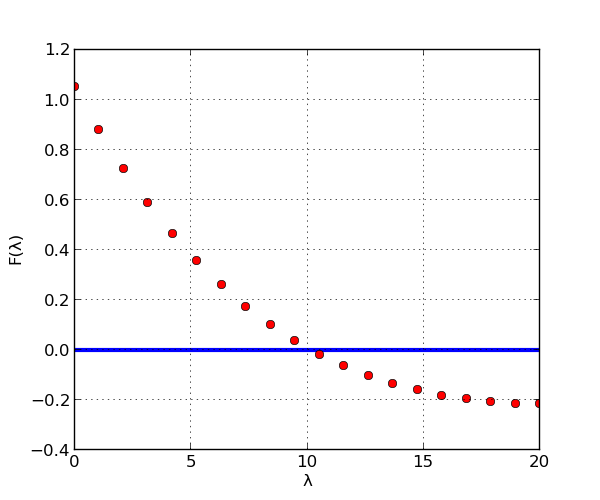
\includegraphics[width=\linewidth]{lambda.png}
  \caption{Зависимость $F(\lambda)$}
\end{figure}

Уточним результат, решив численно уравнение \eqref{eq:dis} с помощью метода секущих, взяв в качестве начального приближения $\lambda_0 = 10$.
В результате получим $\lambda = 10.151184$.

Для полученного $\lambda$ построим решение $u_n(\lambda)$.
Решение изображено на рисунке 2.

\begin{figure}
  \centering
  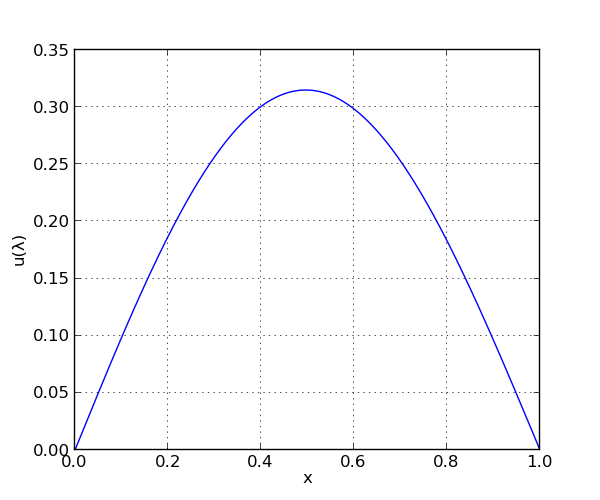
\includegraphics[width=\linewidth]{result.png}
  \caption{Решение $u_n(\lambda)$}
\end{figure}

\end{document}
